\documentclass[../main.tex]{subfiles}
\graphicspath{{img},{img/ink},{ink}}

\begin{document}

\begin{tcolorbox}[
    width=\textwidth,
    height=\textheight,
    title=Phyphox: Federpendel,
    fonttitle=\Large,
    before title=\vspace{0.2cm}, after title=\vspace{0.2cm},
    colback=white,
    title filled=true, 
    colbacktitle=myorange,
    colframe=black,
    coltitle=black,
    ]

    \begin{minipage}[]{0.75\textwidth}
        \vspace{0.2cm}
        \textbf{Klassenstufe}: 9/10 (qualitativ), 11/12 (DGL)

        \vspace{0.5cm}

        \textbf{Fachlicher Bezug}: Pendelbewegung, Schwingung, Bestimmung von Einflussgrößen, Formel der Periodendauer


    \begin{minipage}[]{0.5\textwidth}
        \vspace{0.5cm} 
        \textbf{Material}:
        \begin{itemize}[noitemsep]
            \item Stativmaterial
            \item Meterstab
            \item verschiedene Massestücke
            \item verschiedene Federn
            \item Halterung
            \item Handy + Phyphox
        \end{itemize}
    \end{minipage}
    \hspace{0.45cm}
    \begin{minipage}[]{0.45\textwidth}
        \vspace{0.5cm}
        \includegraphics[width=\textwidth]{img/halterung2}
    \end{minipage}

        \vspace{0.5cm}
        \textbf{Aufbau}: Mit Hilfe des Stativmaterials wird in ausreichender Höhe eine Feder befestigt. In die Feder wird die Halterung mit dem Handy eingehängt. Am unteren Ende der Halterung werden die Massestücke angebracht.
    \end{minipage}
    \hspace{0.3cm}
    \begin{minipage}[]{0.2\textwidth}
        \vspace{0.2cm}
        \includegraphics[width=\textwidth]{img/versuchsaufbau}
    \end{minipage}
 
    \vspace{0.5cm}
    \textbf{Durchführung}: In der Phyphox-App wird \glqq Beschleunigung ohne g\grqq{} ausgewählt. Der Fernzugriff wird aktiviert. Durch Betrachtung der Beschlesunigung in y-Richtung, untersuchen die SuS die Abhängigkeit der Periodendauer $T$ von
    \begin{itemize}[noitemsep]
        \item verschiedenen Auslenkungungen $x$ des Pendel
        \item verschiedenen Massestücken $m$
        \item verschiedenen Federkonstanten $D$
    \end{itemize}
    Die Ergebnisse werden in eine Tabelle eingetragen. Die zusätzliche Berechnung der Größen $\sqrt{m}$ und $\sqrt{\frac{1}{D}}$ wird vorgegeben.

    \vspace{0.5cm}
    \textbf{Ergebnis}: Die Periodendauer $T$ ist unabhängig von der Auslenkung $x$ zu Beginn. Man beobachtet aber die Proportionalitäten
    \begin{align*}
        T \sim \sqrt{m} \\
        T \sim \sqrt{\frac{1}{D}}
    \end{align*}
    
    \vspace{0.5cm}
    \textbf{Didaktische Bemerkungen}: Zur Kontrolle oder nachdem die SuS eigene Beobachtungen gemacht haben, kann in der Phyphox-App unter dem Reiter \glqq Mechanik \grqq{} die Auswahl \glqq Federpendel \grqq{} getroffen werden. Dort wird Periodendauer und Frequenz in der Software berechnet.   
     
\end{tcolorbox}


\end{document}
